\chapter{Introduction}\label{chap:introduction}
% \section{Introduction}
% 2 pages
   \begin{figure}[!ht]
        \centering
        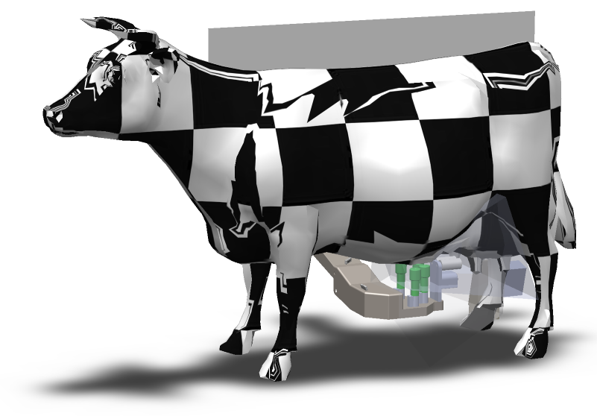
\includegraphics[width=0.65\textwidth]{images/cow_system.png}
        \caption{3D Prototype Model of the Cow Milking Robot}
        \label{fig:cow_fmc}
    \end{figure}
    
\section{Motivation}\label{chap:1:motivation}
% Use Case: Improving the Cow Milking Automation
It is believed that the first time a cow was milked was around 8,000-10,000 years ago, somewhere in Europe\cite{valente_2017}. Interestingly, milk also is given the credit for the developments that have happened in the modern food industry. Not only because of how widespread it is in today's culture, but also because of bringing cheese and butter with it. Over the past 8,000 years, more than a handful of technological advancements have happened, specially in the farming industry. The Agricultural Revolution proved to be a turning point for the food supply, allowing the way for the Industrial Revolution \cite{lumenlearning_2021}. Consequently, milking robots have been around in agriculture for over 20 years. However, the concepts of the widespread milking systems available on the market have hardly had any adaptations leveraging the latest technological advancements. The current largest supplier, Lely, still uses electro-pneumatic spindle motors even in the latest version of the milking robot (Astronaut A5). The benefit of these motors is their low cost and their physical compliance, making them resistant to cow kicks. They require, however, a lot of maintenance. For example, the seal of these motors must be replaced regularly so that the system remains operational. As of today, the herd size in Swiss farms is often big enough so that more than one milking robot would be needed, but the space requirements do not allow for this without having to remodel the barn's infrastructure.

A current project at the ZHAW aims to construct a milking robot that changes the current paradigm, in cooperation with the industrial partner Sutter Landtechnik GmbH (SLG). Most of today's milking robots use a 2D laser scanner to estimate the position of the cow, the udder and the cow's teats. During the position estimation, the robot is static and several measurements are necessary. This is time consuming and if the cow moves during the measurement, the position estimation must be reinitialized. The ZHAW proposes innovative changes to the milking robot's architecture, using electric drives and a more compact kinematic structure. Moreover given the inexpensive 3D cameras have been introduced to the market over the past few years, it is now possible to leverage of high resolution 3D point clouds to dynamically estimate the position of the cow teats.

Based on this background, the aim of this Vertiefungsarbeit (project work) is to select and implement a machine learning and computer vision enabled pipeline that estimates the 3D pose and direction of cow teats. The methods proposed in this work build the basic structure for an approach to estimate the position of the cow teats.

% Although this requires much more complex data processing on a powerful control system, it does away with a time-consuming, separate 
% time-consuming, separate measurement process can be dispensed with. Dynamic measurement with modern sensors also offers the potential to be much more robust and reliable than the measurement methods used today.
    
    % \begin{itemize}
    %     \item describe the general need for automated cow milking
    %     \item describe how the problem is currently being solved briefly
    
    %     \item describe the challenges in cow teat recognition: morphology/shapes and movement
    %     \item describe how these methods fail || describe challenges/limitations of current methods (sensors, etc, no memory)
    
    %     \item can solve this problem with computer vision briefly
    
    %     \item describe cow project main driver (The InIT's purpose) (do we mention how expensive current solutions are?)

    % \end{itemize}
% \section{The Need for Organic Milk}\label{chap:1:organic-milk}

% In recent years, the financial pressure on agriculture in Switzerland has increased massively. Since 1980, the number of farms has been shrinking by about 1000 farms per year. The Swiss consumer wants more and more organically grown products and at the same time consumer prices are getting cheaper and cheaper. The extensive Swiss animal welfare regulations, which are the strictest in Europe, make animal husbandry even more expensive. All this leads to the fact that the average income of a farmer family decreases annually. The farmers' association is therefore calling for greater support from the state. The SLG sees the key to running a profitable Swiss farm not in higher government subsidies, but in a more efficient machine park, which is specifically optimized for the Swiss market, according to Swiss legislation and for organic and ecological farming. All robotic milking equipment available today is not designed for organic farming but optimized to maximize milk yield. However, in the saturated Swiss milk market, what is needed is not more milk, but rather milk produced in a fair, organic and cost-efficient way.

% Across Europe, organically produced milk is still a niche product. However, the SLG is convinced that this will change in the coming years, as consumers in Europe are also paying more and more attention to what they eat and how their food was produced. The focus of a new development should therefore not be on maximizing the amount of milk per animal, but on minimizing investment and operating costs, and above all, these new systems should enable organic farming without compromise. This starts with giving cows access to pastures.

% Today's robotic systems are designed for 24/7 operation. Especially for smaller farms, this mode of operation is necessary to keep operating costs low. In contrast, an important feature of the new robotic system is to be able to milk all cows on a farm within one to two hours, thus combining all the advantages of a conventional milking parlor with the benefits of a milking robot. For this purpose, the new robot is dimensioned in such a way that several robot arms can be installed in the intermediate aisles of existing barns without the need for major cost-intensive building adaptations. By installing the robot in the intermediate aisles of the barn, it will also be possible to minimize the use of concentrated feed, as the cows will automatically pass the robot when moving from the cubicles to the feeding axles.

\section{Related Work}\label{chap:1:related-work}
As mentioned above, laser technology used in the current cow milking robots limits the performance of the systems, which can be improved by leveraging the latest technological advancements. As stated by \textcite{pal2017algorithm}, laser technology is not capable of differentiating between a cow's teat and a leg, therefore manipulating the suction cups in the wrong direction. Along these lines, \citeauthor{pal2017algorithm} propose a fast and reliable solution to the problem of 3D pose recognition of cow teats using TOF, RGBD and Thermal Imaging. 
% Their pipeline provides a new accurate way for estimating the poses but lacks any intelligence with respect to knowing what is a cow teat.
Similarly, \citeauthor{rastogi2019teat} take a stand against the limitations of laser assisted edge detection technologies, which cannot differentiate between a healthy and a diseased teat. They propose two alternatives to the task: a Haar-cascade classifier and a YOLO classifier for cow teats. Both approaches work on real time but lack reliable accuracy. The Haar cadcade classifier fails to detect any teats in the occluded tests, and YOLO fails to detect a fourth teat even with a prediction threshold of 0.5.
% Even though YOLO performs splendidly and even in real-time, YOLO provides only a bounding box for the object found, whereas a segmentation network benefits by separating the pixels of salient object from the background.
Additionally, \textcite{dorokhov2019recognition} analyzed the study from \textcite{akhloufi20143d} for vision systems for livestock and gathered that RGB-D technologies are preferable to ToF. Regardless, they propose a k-nearest neighbors approach from the point cloud captured by a ToF camera. They also state that the vacuum action in the teat attachment step allows for the teat pose estimation error to be at most 1 cm. They fail, however, to provide any benchmarks about the performance of their algorithm.

\textcite{ciocarlie2014towards} propose a complete software achitecture for reliable grasping of household objects. Their work combines scene interpretation from 3D data, grasp planning, motion planning and failure identification and recovery modules. Related to this work, their semantic perception approach uses Eucledian clustering on pre-segmented objects from a scene from a 3D point cloud. They then use a similar technique to the ICP algorithm to match the object clusters to a database of pre-defined 3D models. One of their main concerns for future improvements is that robots should be able to grasp objects in unknown scenarios.

On the same note, \textcite{manuelli2019kpam} state that manipulation policies should generalize to potentially unknown instances. Therefore, they introduce a novel category-level manipulation pipeline that uses semantic 3D keypoints for object representation and enables the specification for robot action planning and grasping with centimeter level precision. 

Finally, \textcite{o20193d} review 3D computer vision systems and techniques for precision dairy farming. More specifically, they look at Time of Flight and streoscopic vision systems. They conclude that robust systems which adapt to weather conditions, herd characteristics, farmyard layout, etc. (generally unknown scenarios) are required. Hence they foresee that the future state of the art technologies use Geometric Deep Learning for processing data in non-Eucledian domain, such as graphs and manifolds. \textcite{cao2020comprehensive} provide a comprehensive review of deep learning methods in the graph and manifold domain, including history, background, applications and benchmark datasets as reference for research in geometric deep learning.

On the similar final note, \textcite{arad2020development} propose an extensively tested and integrated system design for SWEEPER, a robot for harvesting sweet peper fruit in greenhouses. SWEEPER uses time-of-flight technologies and a single sensor for RGB and depth analysis, which combined with a shape and color-based detection algorithm allows high frame-rate operation. To summarize, they use they use traditional-computer-vision-enabled pipeline to analyze the morphology of the shapes recognized, and then compare its relative size to an average pepper size, which allows fast calculations. 
% , which is capable of autonomously driving on irregular floors. 


% 3D vision
\textcite{qi2018frustum} propose, after evaluating a new type of deep net architecture called PointNet\cite{qi2017pointnet}\cite{qi2017pointnet++}, a method that is able to localize objects in large-scene point clouds with high efficiency and high recall, regardless of heavy occlusion or with very sparse points. However their method struggles with multi-instance scenarios, pose estimation accuracy in sparse point clouds, and 3D detection if the 2D detector faces strong occlusion.

to obtain a point cloud of the cow teat  attempt to tackle the problem processing the point cloud 

% \section{Vision Systems in Automated Milking Robots}\label{chap:2:melkroboter}
% half a page

% Vision Systems in Automated Milking Robots

% The systems available on the market all consist of a manipulator and the associated basic equipment. Therefore, when using several manipulators at the same time, the basic equipment must also be present several times. The possibility of operating several manipulators on one base unit (the base unit contains the pumping and cooling units as well as the tanks for the milk) is not in itself a technical-scientific innovation. However, when several manipulators are used, the cost of the individual manipulator plays a significant role in the cost-effectiveness of the overall system. Therefore, the aim is to develop a manipulator that is cost-effective in terms of production, maintenance and operation, using state-of-the-art components. The content of this research project is limited only to the development of a new manipulator. The development of the complete system will be done by SLG outside this research project - the corresponding know-how is available due to years of experience in the development, production and maintenance of own milking systems. The in-house development of the overall system also allows SLG to determine all parameters of the milking process itself and thus adapt them to the specific conditions in Switzerland. The latter is not possible with the systems currently available.

% The robotic milking systems available on the market apply different strategies to detect the cows' teats. The goal is, after the cow has entered the milking parlor and the teats have been hygienically cleaned and stimulated, to apply the teat cups to the teats as quickly as possible. This involves moving the teat cup in front of the teat tip and then moving it in the direction of the teat towards the udder. Due to a vacuum, the teat cup then remains attached to the teat by itself until the vacuum is switched off after the milking process has been completed. Depending on the system, the cup is then removed by pulling back the hose hanging from the cup or by pulling on a separately attached rope.

% The attachment of the four buckets is done in the case of the Lely machines by moving a platform where all four buckets are moved simultaneously until they are attached. This design has the advantage that the
% This design has the advantage that the robot arm only has to travel the long way under the cow once per milking operation, and only short movements are then required for the attachment of the teat cups. In addition, if the cups do not stick to the teat, they fall back onto the platform and not onto the floor, where they become dirty and a time-consuming cleaning process becomes necessary. Thus, the docking time for these systems is typically about one minute for all four cups. However, this design also has drawbacks: The somewhat bulky design means that more volume must be moved between the cows' legs. This is uncomfortable for the cow and also means an increased risk of the cow stepping on or into the robot arm. In addition, the large mass of the platform also means that it is difficult to constantly follow the teat cups to the teat during the docking maneuver. Other products, such as DeLaval's VMS, use the robot to move each cup individually from a magazine next to the cow box to the teat. These manipulators can be built slimmer and lighter, allowing them to move more agilely. The disadvantage is that the docking process for four cups takes longer (about two minutes) and also that if the cup does not adhere properly to the teat, it will fall to the floor under the cow, requiring an additional cleaning procedure.

% The existing milking robots measure the position of the teats once before starting the docking procedure and then approach the teats in a purely position-controlled manner. In contrast, the new manipulator will be designed in such a way that it is able to detect the teats during the entire docking process in order to always be able to move the teat cup in the direction of the teat. This guarantees that even if the cow moves during the docking process, the teat is reached as quickly as possible and with a high degree of safety. In this way, the robustness and also the time of the docking process of the teat cups can be significantly improved. For this, in addition to the appropriate 3D sensor technology, a corresponding real-time evaluation algorithm is required. Furthermore, the manipulator itself must be designed in such a way that it can dynamically move a platform with the four teat cups accordingly. Last but not least, the control system must also be capable of executing sensor-guided movements in real time.

% Even if some competitors have equipped their latest milking robot models with more modern 3D sensors in the meantime, the sensor-guided dynamic target movement described here has not been implemented, among other things because the necessary manipulator design is not available.


\section{Purpose and Research Question}\label{chap:1:research-question}
In this work, a machine learning and computer vision based solution will be used to estimate the pose of cow teats for a milking robot. Regarding this task, this work tackles the following research question:
\begin{itemize}
    \item How can the cow teats 3D pose be estimated under 10 seconds?
\end{itemize}

\section{Approach and Methodology}\label{chap:1:approach-methodology}
This work focuses on computer vision techniques to manipulate RGB-D data to positions and directions of objects in 3D space. The problem that will be solved within this Vertiefungsarbeit is the pose estimation of cow teats.

The planned strategy for this project work is the following:

A state of the art analysis will be done to propose a processing pipeline that answers the research question. This analysis includes the evaluation of a variety of advancements computer vision and machine learning fields such as object segmentation, 3D object recognition, and pose estimation for the 3D pose estimation of cow teats. This also includes the implementations of the proposed algorithms and the respective optimization of their parameters to solve the task optimally. It is also important to note that this process has an iterative nature, where the validation of the models' results will trigger changes in the data sets and the diverse algorithms' parameters, in order to achieve the best possible results. The used data will be of both real and synthetic origins. Finally, the results will be critically evaluated and compared to each other. The reliability and limits of the results will be discussed and further improvements on this field will be considered. 


\section{Scope and Limitation}\label{chap:1:scope}
Due to the time constraints, some limitations have to be laid out to ensure the work can be finished within schedule.
\begin{itemize}
    \item The approach used will focus specifically on the manipulation of RGB-D images, while the manipulation of point clouds will be left out.
    \item This work focuses on the results observed in computer vision and machine learning approaches using 3D cameras. Other techniques, which for example use lasers for 3D scene understanding, will not be taken into account.
    \item This work does not take into account scene understanding and camera manipulation techniques.
    \item This work will focus on the 3D object recognition of cow teats for milking robots.
    % \item 
\end{itemize}
\section{Target Group}\label{chap:1:target-group}
First, this work of special interest for researchers in the field of computer vision. This is due to the fact that 3D object recognition is still a rapidly growing field.  Second, as mentioned in \ref{chap:1:motivation}, the industrial partner Sutter Landtechnik GmbH (SLG) is the private interest group for this research.  This is because SLG not only offers sales, installation and service of technical equipment and machinery for various tasks in agriculture, but also
% It is based in in Andwil and Muolen, Switzerland.
% Its customers are farms of various sizes in German-speaking Switzerland and in nearby foreign countries. 
provides milking technology, which includes milking robots of the "Astronaut" variant\cite{2021lely-a5}.
% , manufactured by the Dutch company Lely. 


% In addition to the areas of tractors and agricultural technology (e.g. harvesting machines), farm technology (barn equipment), there is the area of milking technology, which, in addition to milking machines, includes cooling technology and, last but not least, milking robots. 

% Various machines, including milking technology, were developed by SLG itself and are also manufactured in its own plant. Of the approximately 50,000 farms in Switzerland, about 2,000 are customers of SLG. In addition, there are about 200 farms from nearby foreign countries. With these, SLG generates an annual turnover of ~6.3 MCHF (2018) with its 25 employees. All milking robot systems installed and/or maintained by SLG are of the "Astronaut" type from the Dutch company Lely.

% As the Lely company was not interested in product adaptations for the Swiss market, SLG terminated its direct business relationship with Lely in 2016 and decided to develop its own robotic system. Therefore, in this project, the prototype of a low-cost, modern milking robot suitable for the specific Swiss requirements will be developed, which can be manufactured and marketed by Sutter Landtechnik GmbH (SLG) itself.

% The Lely company with the Astronaut model range has been able to establish itself on the European market for a variety of reasons and is by far the market leader. The European market is dominated by two brands, Lely 55\% and DeLaval 30\% of the market. In Switzerland there are currently around 850 Lely Astronaut and around 300 DeLaval VMS milking robots in operation. The Swiss market is clearly dominated by Lely with a market share of about 72\%. The weak competition, as well as the small Swiss market in relation to Europe, means that specific adaptations only for the Swiss market are not worthwhile for the large groups.
\section{Outline}\label{chap:1:outline}
The following Chapter 2 will cover the theoretical background for this work, making emphasis on computer vision, machine learning approaches, 3D object recognition, and pose estimation. Chapter 3 will describe the methodology, the nature of the data and the pose estimation pipeline's architecture. Chapter 4 will present the achieved results, and chapter 5 will examine the validity and reliability of the presented results. Finally, chapter 6 provides a conclusion and proposes further steps on research for this topic.
% \section{Towards 3D Object Detection}\label{chap:1:detection}

% \lipsum[2-5]

    % \begin{itemize}
    %     \item describe advancements in traditional computer vision for image interpretation
    %     \item list shortcomings/challenges we can overcome with computer vision
        
    %     \item describe advancements in computer vision with DL for object detection
    %     \item list shortcomings/challenges we can overcome with computer vision
        
    %     \item shortcoming1: no object permanence | objects out of sight
    %     \item shortcoming2: reliability of only detecting cow teats (?)
    %     \item HELP: shortcoming3: (?) (need to re-read the papers from gio)

    % \end{itemize}
% \section{Problem Description}\label{chap:1:problem}
% \lipsum[2-3]





% Als Resultat dieses Forschungsprojekts steht der Prototyp eines modernen Melkroboters, welcher durch seine auf kleinere Betriebe angepasste Konstruktion und aufgrund der eigenen Produktion und dem direkten Vertrieb durch SLG auch in kleineren Landwirtschaftsbetrieben rentabel eingesetzt werden kann. Die Forschungsresultate sind für SLG einfach und zeitnah in ein Produkt umwandelbar, welches direkt im Schweizer Landwirtschaftsumfeld vermarktet werden kann und somit im Bereich Landwirtschaft zu einer besseren, effizienteren und ökologischeren Produktion beitragen wird.

    % \begin{itemize}
        % \item in this work we answer the question: ---
        % \item we start by describing:
        %     \SubItem state of algorithms for cow milking
        %     \SubItem state of algorithms for 3d object detection
        %     \SubItem describe the system is able to localize cow teats in 3d space
        %     \SubItem describe the diverse algorithms we evaluated and tested (?)
        %     \SubItem finally we discuss the outcome of experiments and how to interpret conclusions
        %     \SubItem REWRITE/REUSE THIS SENTENCE FROM THESIS: We do not attempt to solve the specific use case of the ZHAW Summit XL Steel mobile robot, but aim to create an approach which is helpful in a large range of possible scenarios, similar to the way 3D mapping systems already enable robotic interaction today.
    % \end{itemize}
